
%(BEGIN_QUESTION)
% Copyright 2013, Tony R. Kuphaldt, released under the Creative Commons Attribution License (v 1.0)
% This means you may do almost anything with this work of mine, so long as you give me proper credit

In this ``inverting'' DC-DC converter circuit, a transistor is alternately switched on and off to control the storage and release of energy in an inductor, thus controlling the average voltage delivered to the load: 

$$\includegraphics[width=15.5cm]{i03493x01.eps}$$

During the transistor's {\it off} period, sketch the following on the schematic diagram:

\begin{itemize}
\item{} Voltage polarity across the inductor (+ and $-$ symbols)
\vskip 5pt
\item{} Voltage polarity across the diode (+ and $-$ symbols)
\vskip 5pt
\item{} Direction of current through the capacitor (arrow pointing in the direction of conventional flow)
\end{itemize}

\underbar{file i03351}
%(END_QUESTION)





%(BEGIN_ANSWER)

$$\includegraphics[width=15.5cm]{i03493x02.eps}$$

%(END_ANSWER)





%(BEGIN_NOTES)

{\bf This question is intended for exams only and not worksheets!}.

%(END_NOTES)

